\section{Messergebnisse und Auswertung}

\subsection{Zählrohrcharakterstik mit \uran}

\begin{figure}[H]
\begin{center}
  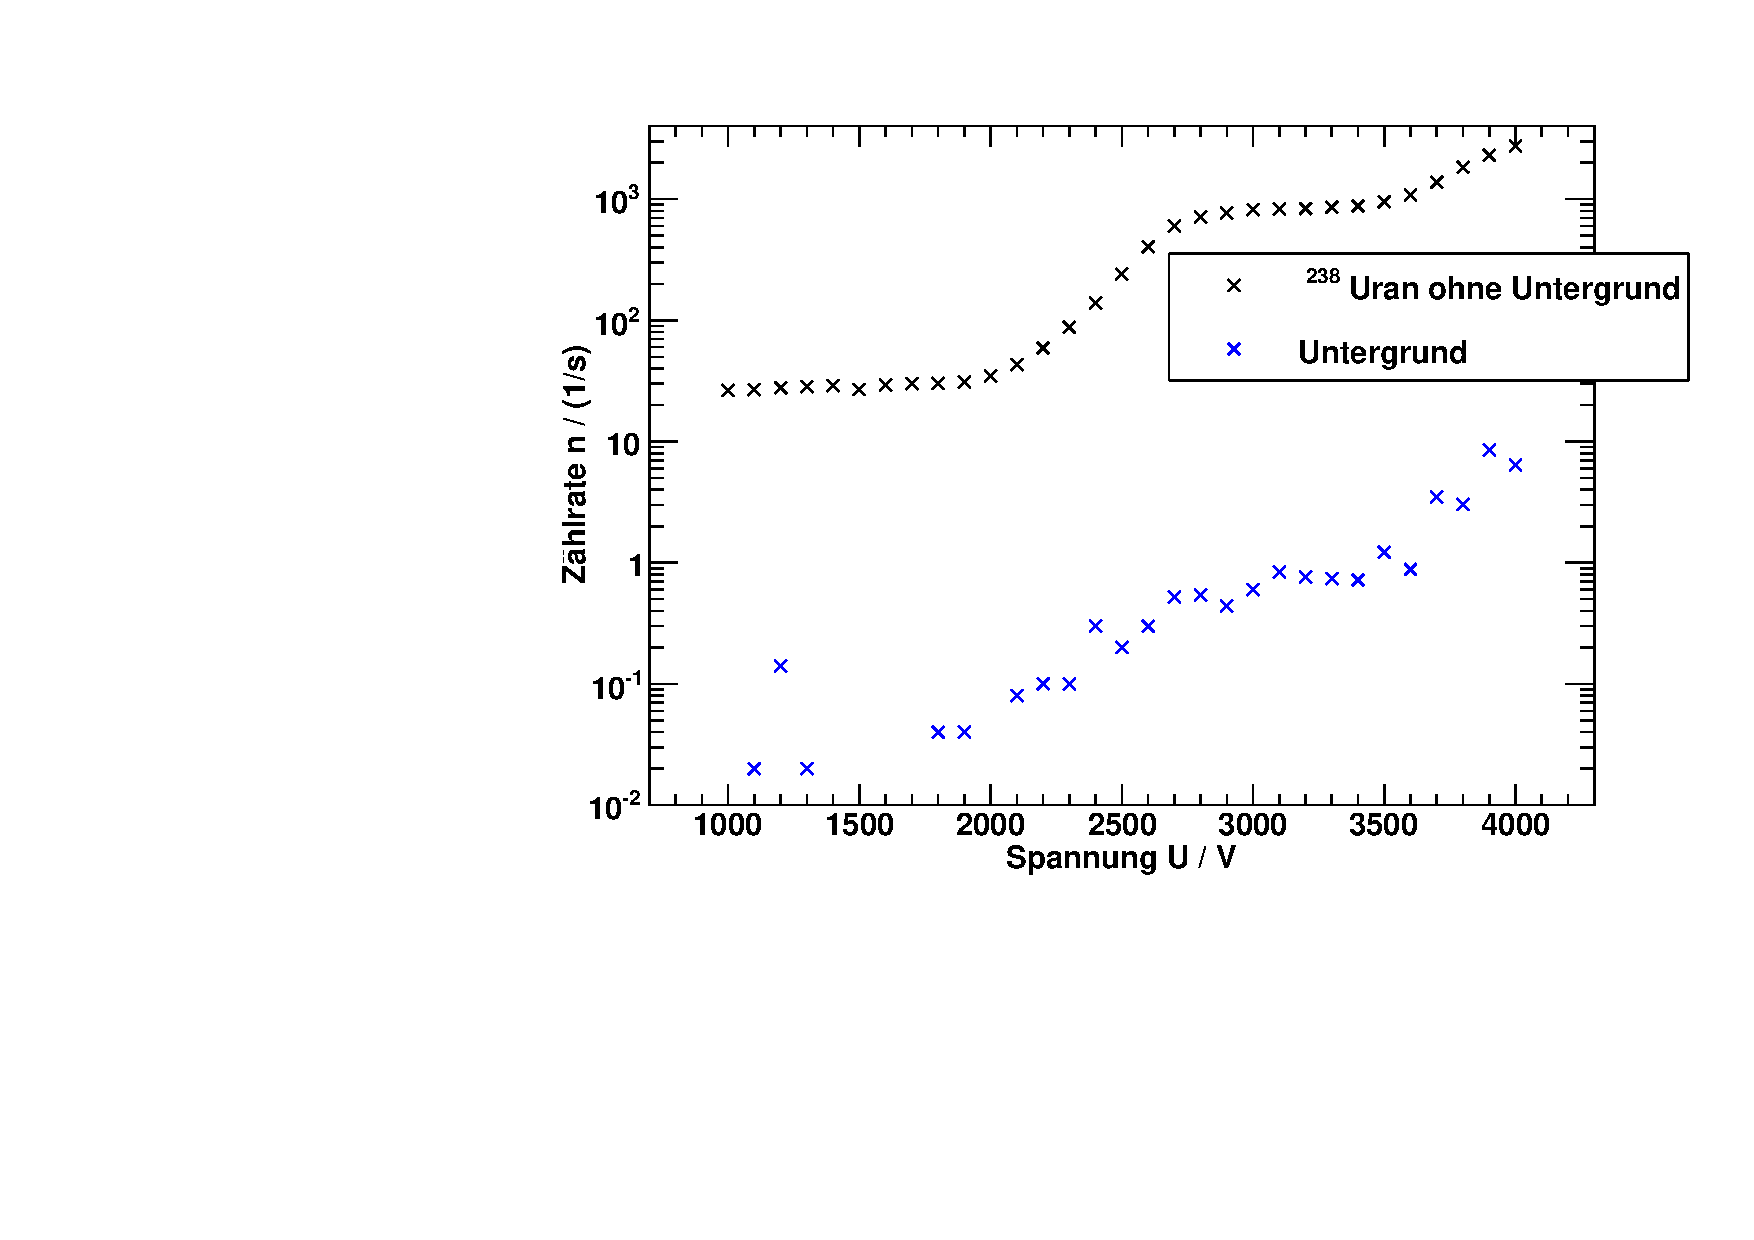
\includegraphics[width=15cm]{../img/Uran238_Charakteristik.pdf}
  \caption[Zählrohrcharakteristik mit \uran]{Zählrohrcharakteristik mit \uran und Untergrund}
  \label{img:char:uran}
\end{center}
\end{figure}
%TODO Beschreibung

\subsection{Bestimmung der Halbwertszeit von \samarium}
\begin{figure}[H]
\begin{center}
  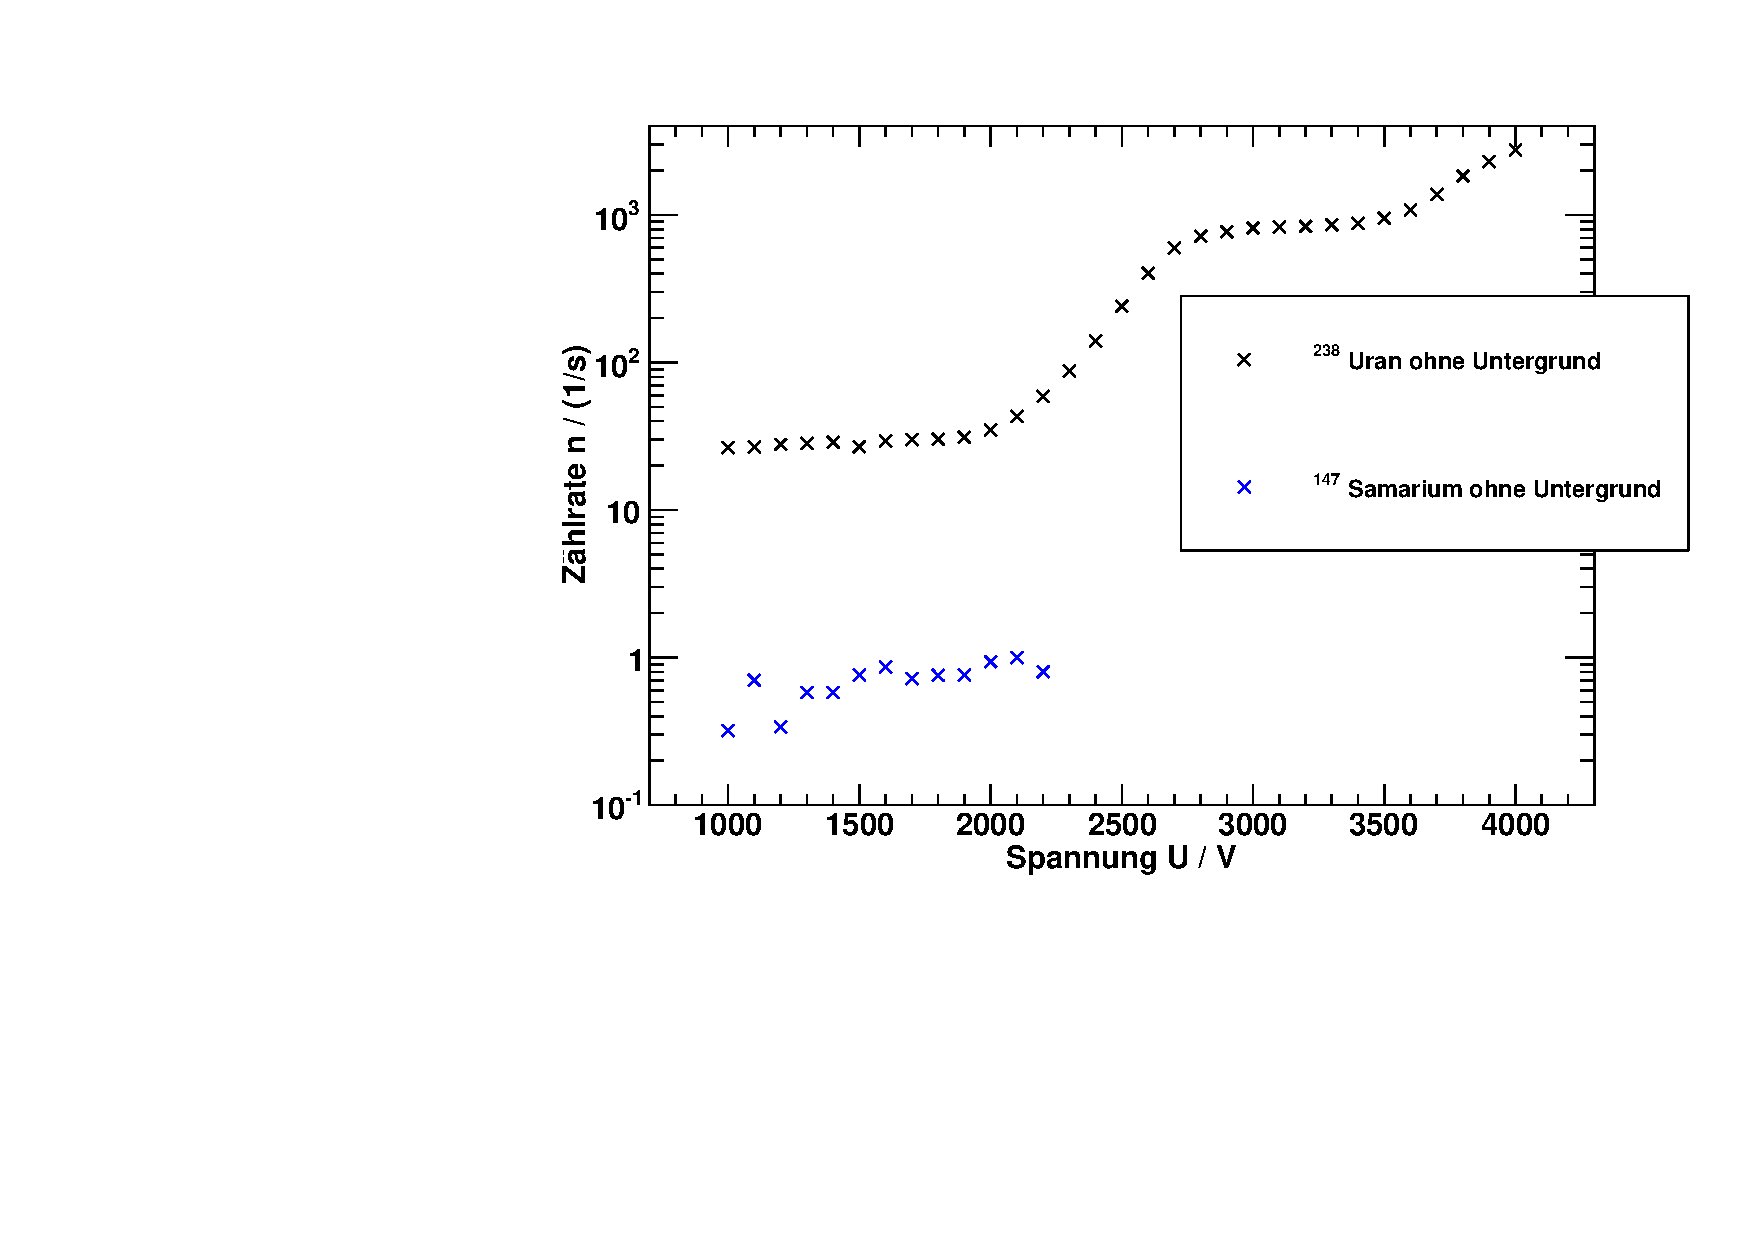
\includegraphics[width=15cm]{../img/Samarium147_Charakteristik.pdf}
  \caption[$\alpha$-Plateau mit \samarium]{$\alpha$-Plateau von \samarium} %TODO bessere beschreibung
  \label{img:char:samarium}
\end{center}
\end{figure}

\begin{figure}[H]
\begin{center}
  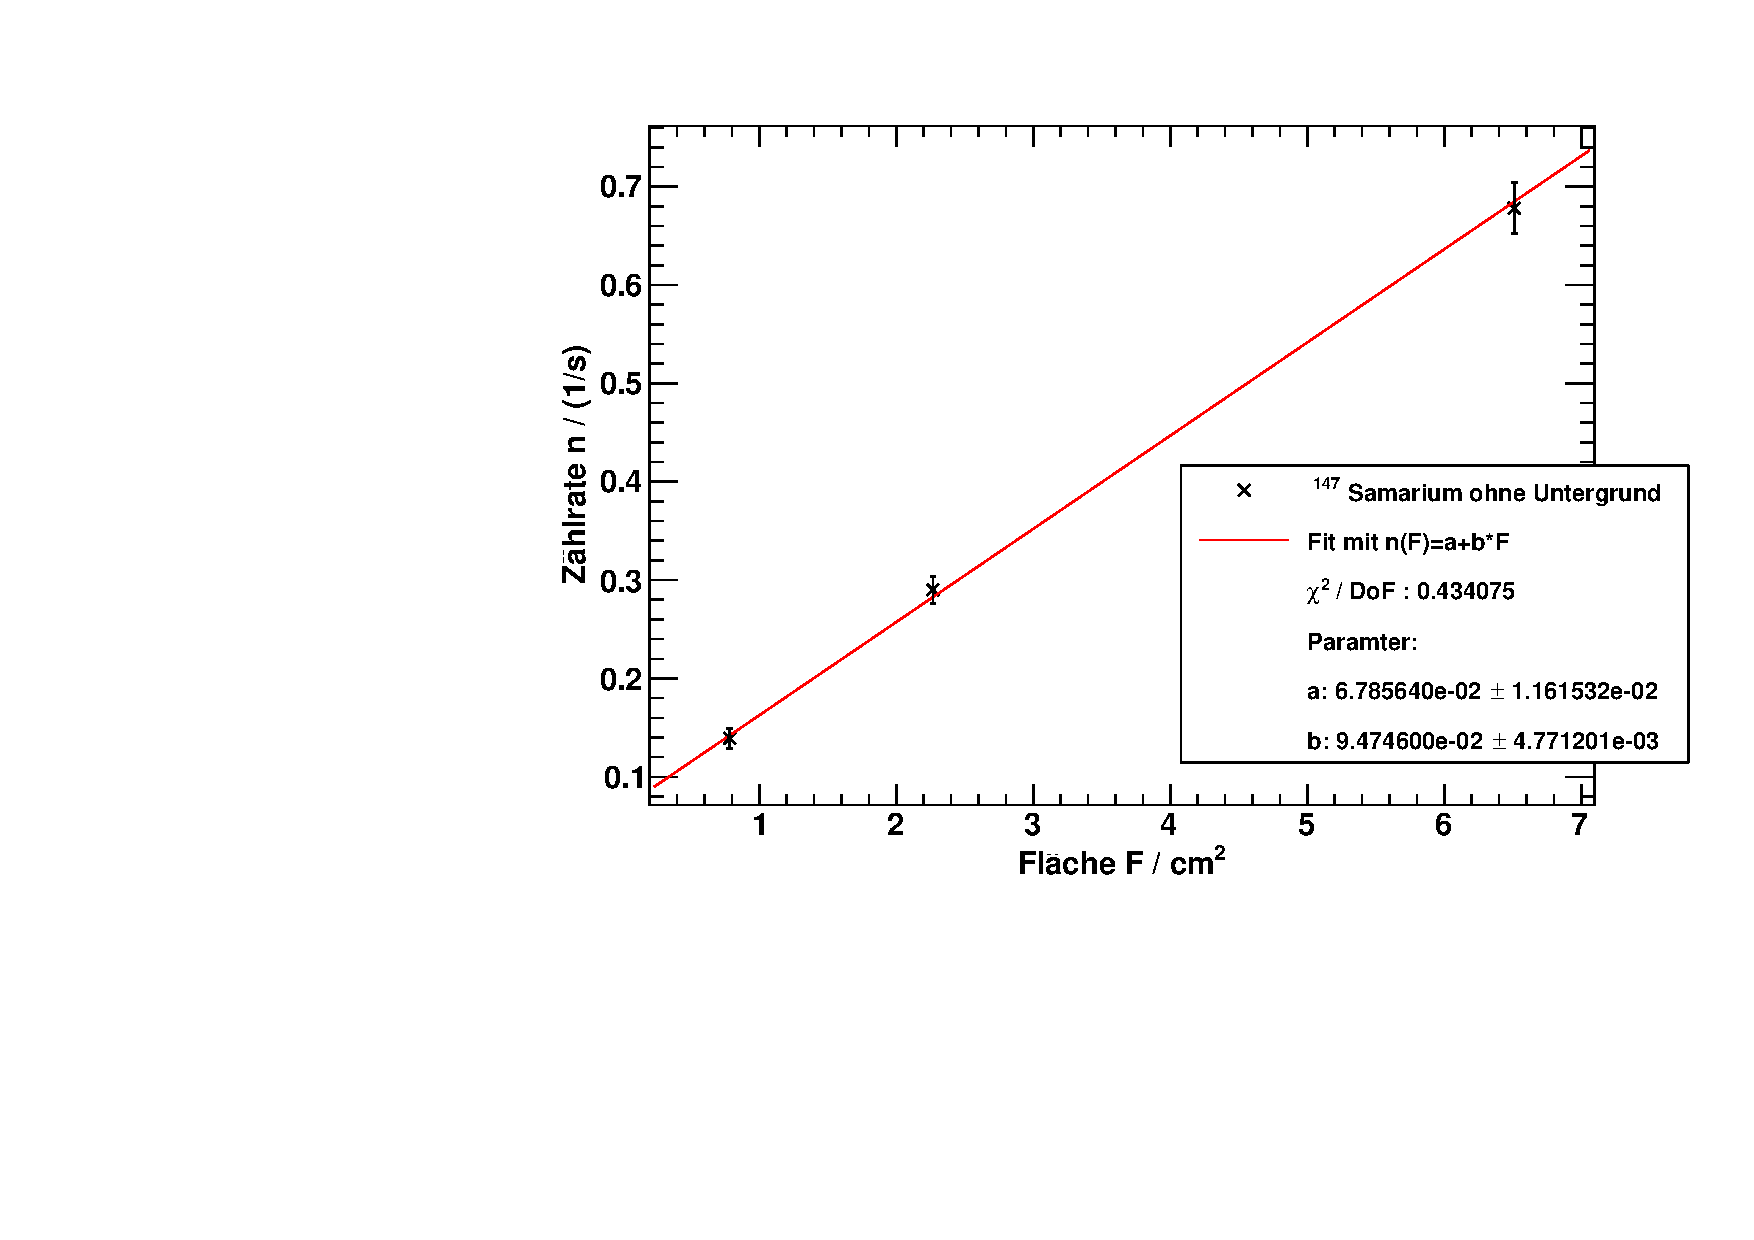
\includegraphics[width=15cm]{../img/Samarium147-Flaechenabhaengigkeit.pdf}
  \caption[Flächenabhängigkeit von \samarium]{Flächenabhängigkeit von \samarium bei 1600V}
  \label{figureLabel}
\end{center}
\end{figure}


%TODO Rest der Samariumauswertung

\subsection{Bestimmung der Halbwertszeit von \kalium}
\subsubsection{$\beta$-Plateau von \kalium}
\begin{figure}[H]
\begin{center}
  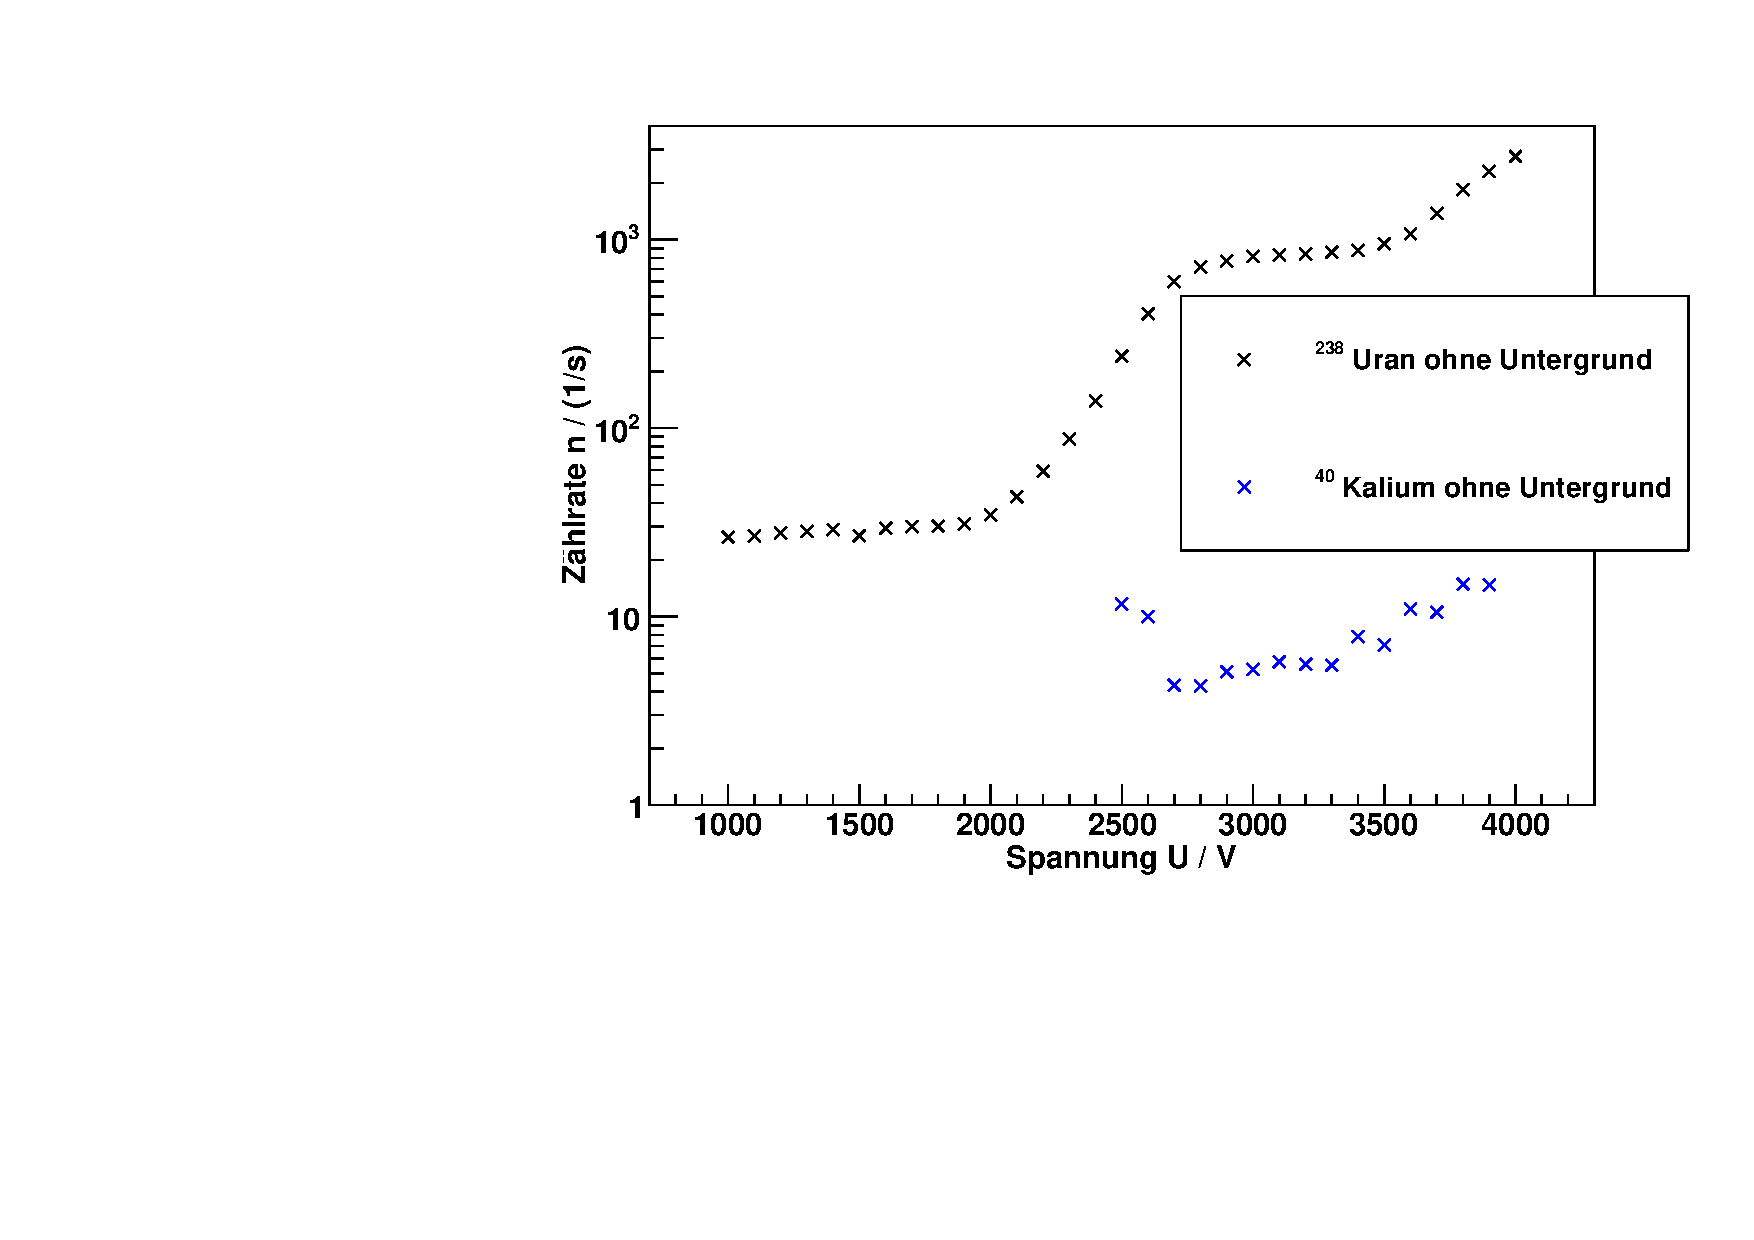
\includegraphics[width=15cm]{../img/Kalium40_Charakteristik.pdf}
  \caption[$\beta$-Plateau mit \samarium]{$\beta$-Plateau von \kalium}
  \label{img:char:kalium}
\end{center}
\end{figure}
%TODO Beschreibung der Graphik

\subsubsection{Massenabhängigkeit der Zählrate} %TODO besserer Titel
Nach * hängt die Zählrate folgendermaßen von der Masse der Probe ab: %TODO \refeq{}
\begin{equation}
  n(m) = \frac{f}{2} \frac{A_s \cdot F \cdot \rho}{\mu} \left( 1 - e^{- \frac{\mu \cdot m}{F \cdot \rho}} \right) = a(1-e^{-b \cdot m})
\end{equation}
mit
\begin{equation}
  a = \frac{f}{2} \frac{A_s \cdot F \cdot \rho}{\mu} \qquad \text{und} \qquad b = \frac{\mu}{F \cdot \rho}
\end{equation}
%TODO Tabelle Messwerte
Die beiden Parameter $a$ und $b$ lassen sich mit einer Kurvenanpassung bestimmen.
\begin{figure}[H]
\begin{center}
  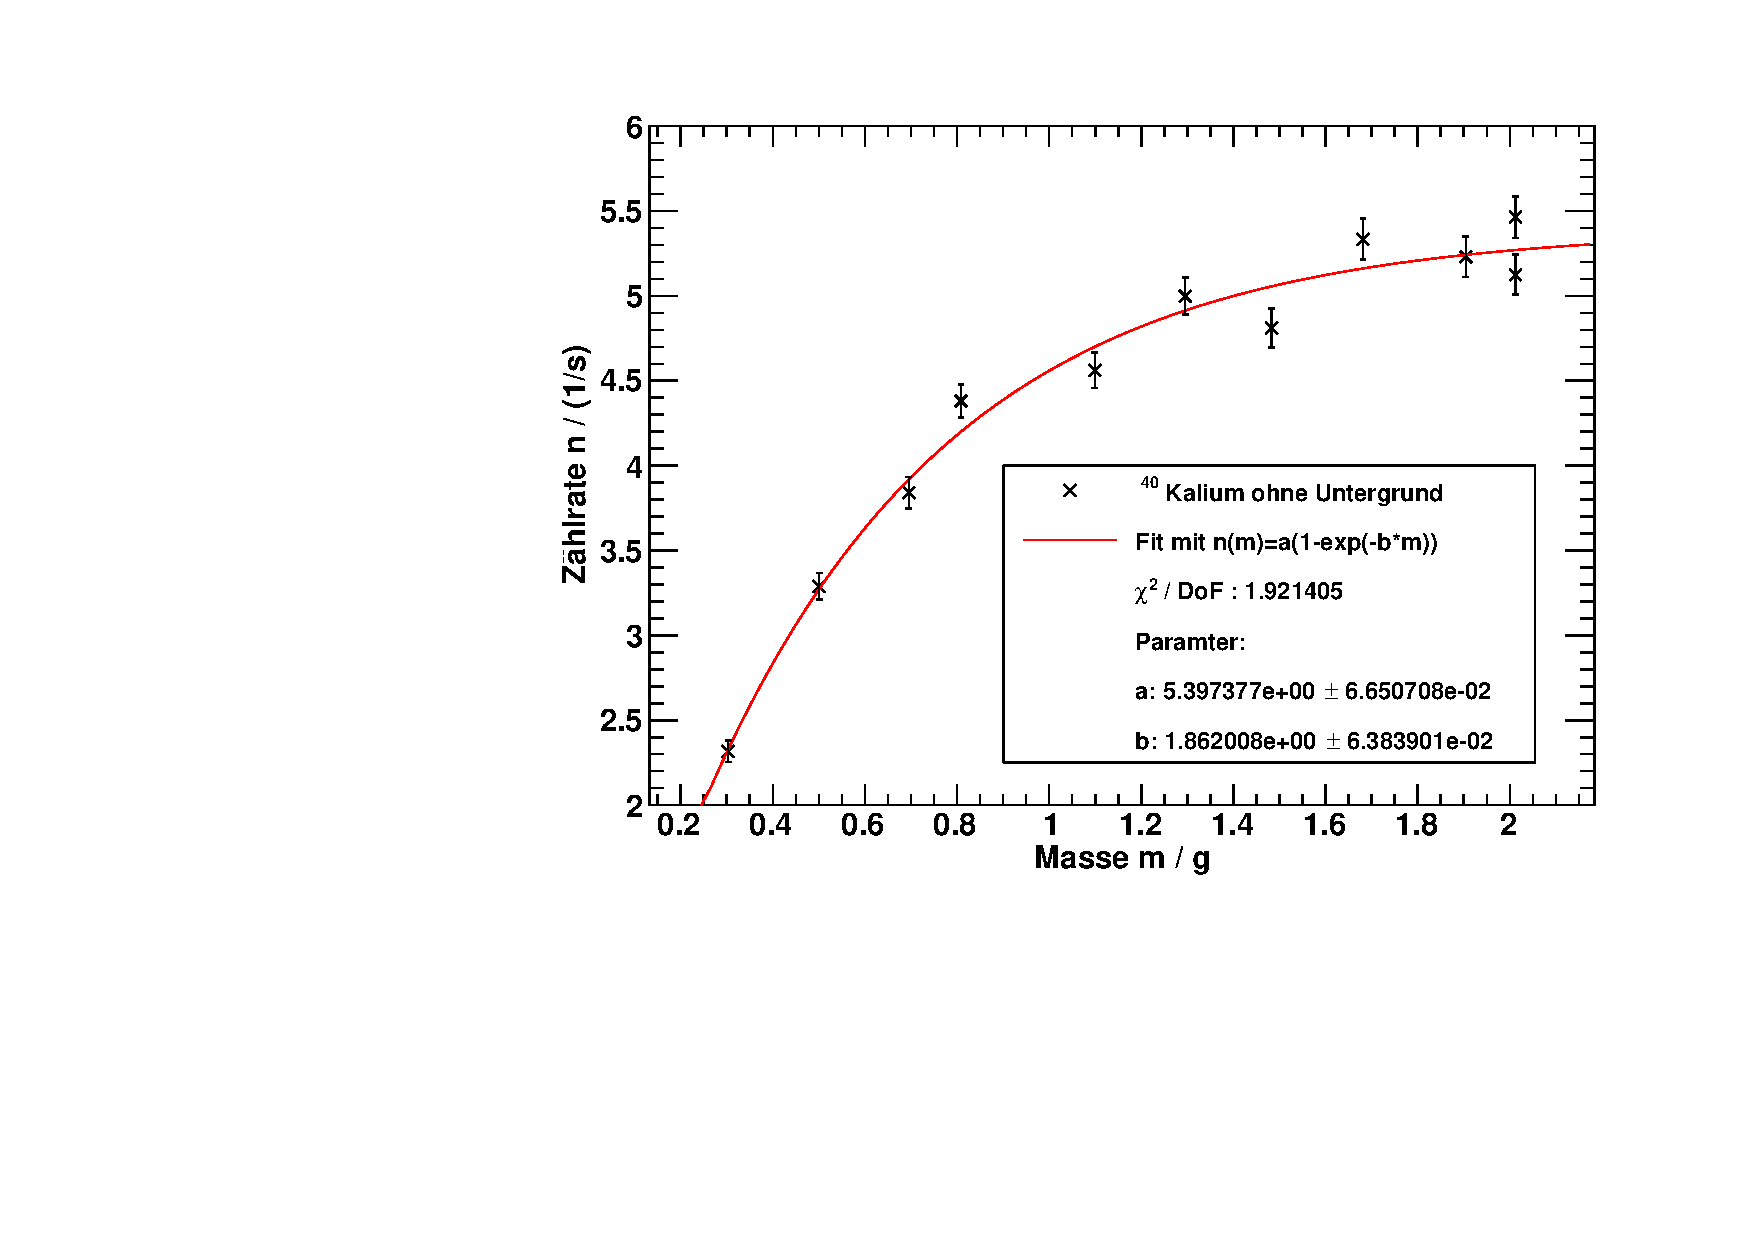
\includegraphics[width=15cm]{../img/Kalium40_Massenabhaengigkeit.pdf}
  \caption[Massenabhängigkeit der Zählrate von \kalium]{Massenabhängigkeit der Zählrate von \kalium bei 3200V}
  \label{figureLabel}
\end{center}
\end{figure}
Die Werte lauten:
\begin{gather}
  a = 5.3973765143 \pm 0.0665070840045 \\ %TODO runden ja oder nein?
  b = 1.86200787667	\pm	0.063839006002
\end{gather}
Außerdem ergibt sich ein Korrelationskoeffizient von
\begin{equation}
  \rho = -0.823206987745
\end{equation}
%TODO Chi^2 / DoF Auswertung

\subsubsection{Berechnung der Halbwertszeit}
Aus dem Produkt der beiden Parameter lässt sich die spezifische Aktivität $A_s = \frac{A}{m}$ bestimmen:
\begin{equation}
  A_s = \frac{2 \cdot a \cdot b}{f}
\end{equation}
Die Halbwertszeit von Kalium lässt sich nach * mit %TODO refeq
\begin{equation}
  T_{1/2}({}^{40}K) = \frac{\ln 2}{1.12} \frac{N}{A}
\end{equation}
bestimmen. \\
Die Anzahl $N$ der Kaliumkerne in Kaliumchlorid ist:
\begin{equation}
  N = \frac{m \cdot N_A}{M_{KCl}} h_{\text{rel}}
\end{equation}
wobei $N_A$ die Avogadrokonstante, $M_{KCl}=74.5483\,u$ die molare Masse von Kaliumchlorid und $h_{\text{rel}}=0.0118\%$ die relative Anzahl von Kaliumkernen 
in Kaliumchlorid ist. \\
Daraus berechnet sich die Halbwertszeit von Kalium mit:
\begin{equation}
  T_{1/2} \left( {}^{40} K \right)  = \frac{\ln 2}{1.12} \frac{N_A \cdot h_{\text{rel}}}{M_{KCl}} \frac{f}{2} \frac{1}{a \cdot b} = const. \cdot \frac{1}{a \cdot b}
\end{equation}
Der Fehler ergibt sich aus den relativen Fehlern von $a$ und $b$ und der Berücksichtigung des Korrelationskoeffizienten $\rho$:
\begin{equation}
  \sigma_{T_{1/2}} = \sqrt{ \left( \frac{\sigma_a}{a} \right)^2 + \left( \frac{\sigma_b}{b} \right)^2 + 2 \cdot \frac{\sigma_a}{a} \cdot \frac{\sigma_b}{b} \cdot \rho   }
\end{equation}
Man erhält folgendes Ergebnis:
\begin{equation}
  T_{1/2} \left( {}^{40} K \right) = (1.199786 \pm 0.03015611) \cdot 10^9\,a \approx (1.20 \pm 0.03) \cdot 10^9\,a  
\end{equation}

%Tabellen mit Messergebnissen
%Abbildungen
%Auswertung, in der die Analyse der Messdaten beschrieben wird und die Ergebnisse mit ihren Fehlern zusammengestellt werden.